\section{Zielsetzung}

Ziel dieses Versuches ist es, mithilfe eines Michelson-Interferometer die Wellenlänge
eines Lasers zu bestimmen sowie über Druckvariation den Brechungsindex von Luft zu bestimmen.

\section{Theorie}
\label{sec:Theorie}

\subsection{Kohärentes Licht}

\subsection{Michelson Interferometer}
\label{sec:Michelson Interferometer}

Der schematische Aufbau des 1882 von A. Michelson erfundenen Michelson-Inteferometer ist in
\autoref{fig:Michelson} dargestellt.

\begin{figure}[H]
    \centering
    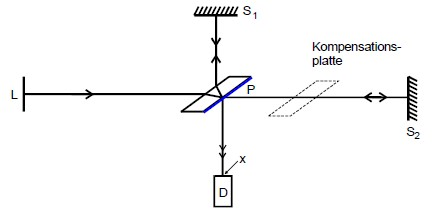
\includegraphics[height=6cm]{content/pics/Michelson.jpg}
    \caption{Schematischer Aufbau eines Michelson Interferometers \cite{v401}.}
    \label{fig:Michelson}
\end{figure}

Der Lichtstrahl aus einer Quelle L wird zuerst durch eine semipermeable Platte P geteilt und somit in zwei Bündel gespalten,
welche sich senkrecht zueinander weiterbewegen.
Die beiden Teilbündel fallen auf zwei Spiegel $\text{S}_1$ und $\text{S}_2$ und werden zurückgeworfen.
Somit treffen die Strahlen wieder in P aufeinander.
Von jedem Strahl wird jeweils ein Teil transmittiert, diese Teilbündel laufen abschließend parallel zueinander zum
Detektor D.


\subsection{Druckabhängigkeit des Brechungsindex}

Die Lichtwellen im Inteferometer werden auch durch die Luft, die sich überall im Interferometer befindet,
gebrochen. Bei den vorherigen Betrachtungen ist der Luftdruck konstant, daher hat diese Tatsache
keinen Einfluss auf die Funktionsweise des Inteferometers.
Wird jedoch der Druck variert, so ändert sich der Brechungsindex $n$ in Luft und damit auch die Interferenz.
Der neue Brechungsindex lässt sich unter Normalbedingungen ($p_0=\qty{1013.2}{\milli\bar}$ und $T_0=\qty{273.15}{\kelvin}$)
über die folgende Beziehung berechnen

\begin{equation}
    \label{eq:Brechung}
    n(p_0, T_0) = 1 + \symup{\Delta} n(p,p')\frac{T}{T_0}\frac{p_0}{p - p'}.
\end{equation}

Dabei ist die Änderung des Brechungsindex $\symup{\Delta} n(p,p')$ bereits in \autoref{sec:Michelson Interferometer} mit
\eqref{eq:Delta N} definiert worden.